\chapter*{ВВЕДЕНИЕ}                         % Заголовок
\addcontentsline{toc}{chapter}{ВВЕДЕНИЕ}    % Добавляем его в оглавление

\paragraph*{Актуальность проблемы}
Язык программирования - основной инструмент любого разработчика. От его эргономики, то насколько легко на нем излагать идеи, напрямую зависит продуктивность разработчка.
В случае языка

На практике часто встречаются задачи, когда стандартных утилит для работы с языком недостаточно, и приходится писать свои собственные.
Цель данного проекта - помочь в разработке подобных утилит.

Разработчику предлагается использовать данную библиотеку для превращения программного кода в абстрактное синтаксическое дерево - 
структуру данных, которая может быть обработанно процедурно (программным путем).

% TODO
Си это язык со слабой статической типизацией.

\def\titlecite#1{\citetitle{#1}\cite{#1}}

\paragraph*{Постановка задачи}
Изучить стандарты\cite{c99_std}\cite{c23_std} языка Си.

Организовать интерфейс для данной библиотеки с помощью абстракции "Единицы трансляции" (Translation Unit)\cite{wiki-tr-unit}.

% \textbf{ecc} является source-to-source компилятором, т.е.компилятором, транслирующих текст программы на одном языке программирования в текст программы 
% на другом (возможно том же самом) языке программирования. 
% В данном случае после разбора текста синтаксическая надстройка на Си интерперетируется, после чего полученное в ходе интерпретации дерево компилируется к тексту языка Си.

Идея состоит в том, чтобы часть функционала компилятора Си, вынести в виде пользовательской библиотеки.
Необходимость такого функционала возникает, когда у разрабочка возникает потребность 

Си устоявшийся(stable) и стандатизированный язык, 
поэтому нет проблемы нестабильного API из-за постоянно развивающего языка, как например сейчас происходит в Rust.

\subsection*{Обзор литературы}

\titlecite{c23_std}, \titlecite{c99_std} - основные документы, содержащие информацию о языке Си.

\titlecite{crafting_interpreters} - основная книга, использованная в данной работе. 
В ней продемострирован метод рекурсивного спуска, описан лексер и парсер для придуманного автором языка Lox.
На основе главы этой книги была написана имлементация хэш-таблицы, использованной в данной работе[\ref{prim:hashmap}].

\titlecite{hmu} - теория формальных языков, абстрактных вычислительных машин и грамматик. 
Данная книга использовалась как источник математического знания по теме на ранних этапах изучения.

\textit{The Theory of Parsing, Translation, and Compiling (Volume I, II)}
\cite{ptc_vI} \cite{ptc_vII} - классические книги по теории компиляции.

\titlecite{monparsing_paper}\titlecite{ml_syntax_transformation_paper} - статьи про монадические парсеры.

\titlecite{peg_paper} - оригинальная статья автора PEG грамматики.

\paragraph{Разбор выражений и приоритет операций}
% \caption{pratt}
\label{litover:pratt} \mbox{} \\
\titlecite{tdop_pratt_paper} - оргинальная статья автора \\
\titlecite{nystrom_pratt_parsers} - поясняющая статья с упором на практику \\
\titlecite{cppref_op_prec} - справка по языку Си: приоритет операций \\
\titlecite{pest_op_pratt} - парсер Пратта в фреймворке pest

% \paragraph*{Актуальность темы.}


% \paragraph*{Цель работы.}

% \paragraph*{Задачи работы.}

% \paragraph*{Научная новизна работы.}

% \paragraph*{Теоретическая и практическая значимость работы.}

% \paragraph*{Положения выносимые на защиту.}
% \begin{enumerate}
%     \item \statementOneRU
%     \item \statementTwoRU 
% \end{enumerate}

% \paragraph*{Апробация работы.}

% \paragraph*{Достоверность научных достижений.}

% \paragraph*{Внедрение результатов работы.}

% \paragraph*{Публикации.} Список всех публикаций автора по теме диссертации:
% \begin{refsection}[biblio/own.bib]
% \nocite{*}
% \printbibliography[
%     keyword=own,
%     %title={Список всех публикаций автора по теме диссертации}, 
%     %heading=subbibliography,
%     heading=none,
%     resetnumbers=true
% ]
% \end{refsection}



% \paragraph*{Структура и объем диссертации. }
% Диссертация состоит из~введения,
% \formbytotal{totalchapter}{глав}{ы}{}{},
% заключения и
% \formbytotal{totalappendix}{приложен}{ия}{ий}{}.
% %% на случай ошибок оставляю исходный кусок на месте, закомментированным
% %Полный объём диссертации составляет  \ref*{TotPages}~страницу
% %с~\totalfigures{}~рисунками и~\totaltables{}~таблицами. Список литературы
% %содержит \total{citenum}~наименований.
% %
% Полный объём диссертации составляет
% \formbytotal{TotPages}{страниц}{у}{ы}{}, включая
% \formbytotal{totalcount@figure}{рисун}{ок}{ка}{ков} и
% \formbytotal{totalcount@table}{таблиц}{у}{ы}{}.
% Список литературы содержит
% \formbytotal{citenum}{наименован}{ие}{ия}{ий}.


% \begin{figure}
%     \centering
%     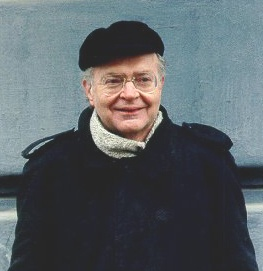
\includegraphics[width=0.6\linewidth]{images/knuth}
%     \caption{Knuth}
%     \label{fig:my_label}
% \end{figure}